\documentclass{beamer}
\usetheme{CambridgeUS}

\setbeamertemplate{caption}[numbered]{}

\usepackage{enumitem}
\usepackage{tfrupee}
\usepackage{amsmath}
\usepackage{amssymb}
\usepackage{textcomp, gensymb}
\usepackage{graphicx}
\usepackage{txfonts}
                               
\providecommand{\pr}[1]{\ensuremath{\Pr\left(#1\right)}}
\providecommand{\mbf}{\mathbf}
\providecommand{\qfunc}[1]{\ensuremath{Q\left(#1\right)}}
\providecommand{\sbrak}[1]{\ensuremath{{}\left[#1\right]}}
\providecommand{\lsbrak}[1]{\ensuremath{{}\left[#1\right.}}
\providecommand{\rsbrak}[1]{\ensuremath{{}\left.#1\right]}}
\providecommand{\brak}[1]{\ensuremath{\left(#1\right)}}
\providecommand{\lbrak}[1]{\ensuremath{\left(#1\right.}}
\providecommand{\rbrak}[1]{\ensuremath{\left.#1\right)}}
\providecommand{\cbrak}[1]{\ensuremath{\left\{#1\right\}}}
\providecommand{\lcbrak}[1]{\ensuremath{\left\{#1\right.}}
\providecommand{\rcbrak}[1]{\ensuremath{\left.#1\right\}}}
\providecommand{\abs}[1]{\vert#1\vert}
\newcommand*{\permcomb}[4][0mu]{{{}^{#3}\mkern#1#2_{#4}}}
\newcommand*{\perm}[1][-3mu]{\permcomb[#1]{P}}
\newcommand*{\comb}[1][-1mu]{\permcomb[#1]{C}}

\newcounter{saveenumi}
\newcommand{\seti}{\setcounter{saveenumi}{\value{enumi}}}
\newcommand{\conti}{\setcounter{enumi}{\value{saveenumi}}}

\makeatletter
\newenvironment<>{proofs}[1][\proofname]{%
    \par
    \def\insertproofname{#1\@addpunct{.}}%
    \usebeamertemplate{proof begin}#2}
  {\usebeamertemplate{proof end}}
\makeatother

\title{Assignment 10}
\author{Kotikalapudi Karthik (CS21BTECH11030)}
\date{\today}
\logo{\large \LaTeX{}}


\begin{document}

% Title page frame
\begin{frame}
    \titlepage 
\end{frame}

% Remove logo from the next slides
\logo{}


% Outline frame
\begin{frame}{Outline}
    \tableofcontents
\end{frame}

%Question
\section{Question}
\begin{frame}{Question}
    \begin{block}{Probability, Random Variables and Stochastic Processes Chapter 2, Problem 2-25} 
        A train and a bus arrive at the station at random between $9$ A.M. and $10$ A.M. The train stops for 10 minutes and the bus for x minutes. Find x so that the probability that the bus and the train will meet equals $0.5$
    \end{block}
\end{frame}

%Solution
\section{Solution}
\begin{frame}{Solution}
\begin{block}{}
    Let's denote the random variable $X_1$ map to the set $\cbrak{0,1}$ where $X_1 = 0$ denote that bus and train don't meet and $X_1=1$ denote that they meet.
\end{block}
\begin{block}{}
    Let's denote the random variable $X_2$ map to the set $\cbrak{0,1}$ where $X_2 = 0$ denote that bus arrives first and $X_2=1$ denote that train arrives first.
\end{block}
\end{frame}

\section{Method-I}
\begin{frame}{Method-I}
    Given, train stops for 10 mins and bus stops for $x$ minutes.\\
    Let's draw a graph with Arrival time of bus in mins on X-axis and Arrival time of train in mins on Y-axis.\\
    For the region in which bus and train meet(in blue color),\\
    $Y<X+x$(train should arrive within $x$ minutes after the bus) and
    $X<Y+10$(bus should arrive within 10 minutes after the train)
\end{frame}

\begin{frame}{Graph}
    \begin{figure}[!ht]
		\centering
		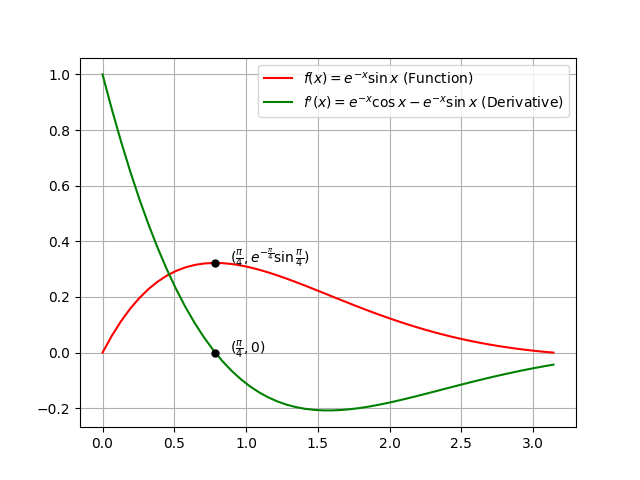
\includegraphics[width=\textwidth,height=5.5cm,keepaspectratio]{Figure_1.png}
		\caption{Arrival times of Bus and train}
		\label{fig:fig1}
	\end{figure}
\end{frame}

\begin{frame}{Finding the Value of x}
    \begin{align}
        \text{Given, }\pr{X_1=1} &= 0.5\\
        \implies \pr{X_1=0} &= 0.5
        \label{eq:eq-1}
    \end{align}
    Substituting the values from the Figure \eqref{fig:fig1} in equation \eqref{eq:eq-1},
    \begin{align}
        \frac{\frac{1}{2}\sbrak{\brak{60-x}^2+50\times50}}{60\times60} &= 0.5
        \\
        \implies \brak{60-x}^2+50\times50 &= 60\times60
        \\
        \implies \brak{60-x}^2 &= 1100
        \\
        \implies x &= 60 - 10\sqrt{11} \approx 26.83 \text{ mins}
    \end{align}
\end{frame}

\section{Method-2}
\begin{frame}{Method - II}
    Let the bus arrive at time $t_B$ and train at $t_T$.\\
    Let's take the area $1 min^2$ as $1$ unit
    \begin{align}
        \implies n\brak{\Sigma^{1}_{i=0}X_1=i} &= \int_{0}^{60} \brak{\int_{0}^{60} \,dt_T}\,dt_B
        \\
        &= 3600
    \end{align}
    If train arrives first, it can arrive in first $50$ mins or last $10$ mins.\\
    If train arrives in first $50$ mins, for each value of $t_T$, bus should arrive within $t_T+10$ mins.\\
    It train arrives in $50$ to $60$ mins, for each value of $t_T$, bus should arrive within $60$ mins.\\
    \begin{align}
        \implies n\brak{X_1=1,X_2=1} &= \int_{0}^{50} \brak{\int_{t_T}^{t_T+10} \,dt_B} \,dt_T + \int_{50}^{60} \brak{\int_{t_T}^{60} \,dt_B} \,dt_T
    \end{align}
\end{frame}

\begin{frame}{If Bus arrives first}  
    If bus arrives first, it can arrive in $60-x$ mins or last $x$ mins.\\
    If bus arrives in first $60-x$ mins, for each value of $t_B$, train should arrive within $t_B+10$ mins.\\
    It bus arrives in $60-x$ to $60$ mins, for each value of $t_T$, train should arrive within $60$ mins.\\
    \begin{align}
        \implies n\brak{X_1=1,X_2=0} &= \int_{0}^{60-x} \brak{\int_{t_B}^{t_B+x} \,dt_T} \,dt_B + \int_{60-x}^{60}\brak{\int_{t_B}^{60} \,dt_T} \,dt_B
        \\
        \text{Also, }n(X_1=1) &= n\brak{X_1=1,X_2=0}+n\brak{X_1=1,X_2=1}
    \end{align}
    
\end{frame}

\begin{frame}{If Bus and train meet}
   \begin{align}
       n(X_1=1) &= 500+x\brak{60-x}+\int_{50}^{60}(60-t_T) \,dt_T + \int_{60-x}^{60}(60-t_B)\,dt_B
       \\
       &= 1100 + 120x -x^2-\int_{50}^{60}t_T \,dt_T - \int_{60-x}^{60}t_B\,dt_B
       \\
       &= 1100 + 120x -x^2-\brak{\frac{60^2-50^2}{2}}-\brak{\frac{60^2-\brak{60-x}^2}{2}}\\
       &= \frac{1100+120x-x^2}{2}
    \end{align}
    \begin{align}
       \implies |n\brak{X_1=1}| &= \frac{\brak{60-x}^2+2500}{2}
    \end{align} 
\end{frame}

\begin{frame}{Finding the Value of x}
We know that,
   \begin{align}
       \pr{X_1=1} &= \frac{n\brak{X_1=1}}{n\brak{\Sigma^{1}_{i=0}X_1=i}} = 0.5
       \\
        \frac{\frac{1}{2}\sbrak{\brak{60-x}^2+50\times50}}{60\times60} &= 0.5
        \\
        \implies \brak{60-x}^2+50\times50 &= 60\times60
        \\
        \implies \brak{60-x}^2 &= 1100
        \\
        \implies x &= 60 - 10\sqrt{11} \approx 26.83 \text{ mins}
    \end{align} 
\end{frame}

\end{document}